\section{Theorie}
\label{sec:Theorie}

\subsection{Einleitung}
Das Geiger-Müller-Zählrohr wird zur Messung der Intensität ionisierter Strahlung verwendet.
Wird ein $\alpha$, $\beta$ oder $\gamma$ - Teilchen absorbiert, so wird ein Impuls erzeugt.
Die Anzahl der Impulse pro Zeit- und Flächeneinheit werden mithilfe eines Impulszählers gemessen.

\subsection{Aufbau und Wirkungsweise}
Der Aufbau eines Geiger-Müller-Zählrohr ist in Abb. \ref{fig:geiger} skizziert.
Innerhalb eines Kathodenzylinder mit Radius $r_k$ befindet sich ein axial verlaufender Anodendraht mit Radius $r_a$.
Der Zylinder ist mit einem Gasgemisch gefüllt.
Wird eine Spannung angelegt, so entsteht ein radialsymmetrisches Feld zwischen Anode und Kathode.
\begin{figure}
    \centering
    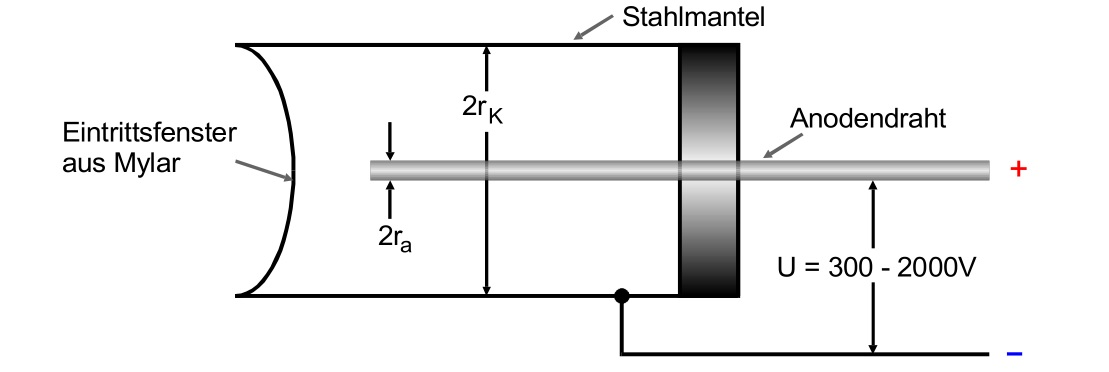
\includegraphics[width=0.8\textwidth]{content/data/geiger.jpg}
    \caption{Aufbau eines Geiger-Müller-Zählrohr. \cite[1]{anleitung}}
    \label{fig:geiger}
\end{figure}
Befindet sich ein gelades Teilchen in dem elektrisches Feld, so wächst das Feld in Richtung des Drahtes mit $\frac{1}{r}$.
Trifft ein Teilchen in das Zählrohrvolumen, so wird es sich im Gasraum bewegen, bis die Energie durch Ionisationsakte aufgebraucht ist.
Die Anzahl der dabei entstehenden Elektronen bzw. positiven Ionen ist proportional zur Energie des einfallenden Teilchens.
Wie in Abb. \ref{fig:spannung} zu sehen, hängt die Ionisation im Zählrohr von der angelegten Spannung ab.
\begin{figure}
    \centering
    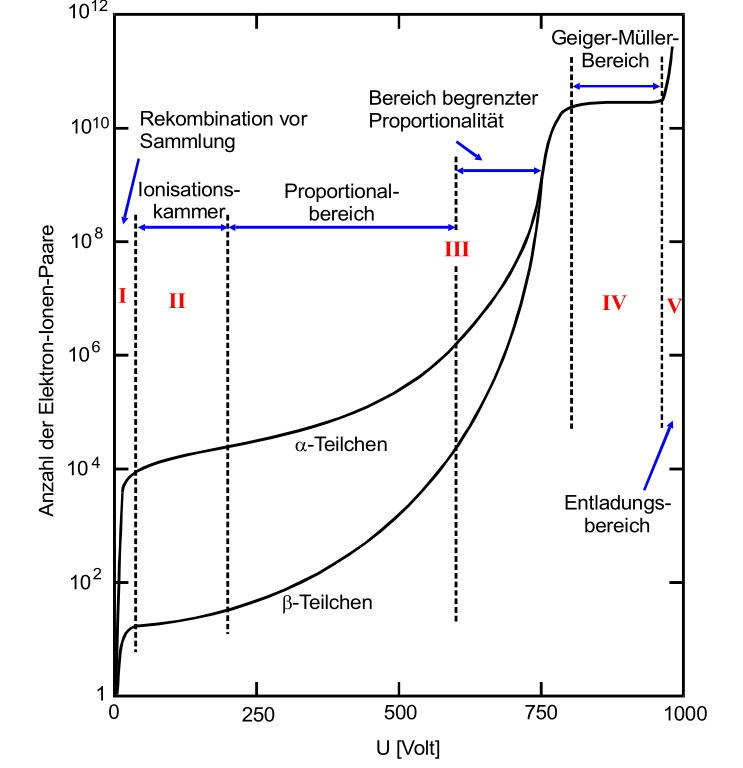
\includegraphics[width=0.6\textwidth]{content/data/spannung.jpg}
    \caption{Anzahl der erzeugten Elektron-Ionenpaare in Abhängigkeit der Spannung $U$. \cite[2]{anleitung}}
    \label{fig:spannung}
\end{figure}
\\
Bei geringer Spannung (Bereich I) erreicht nur ein geringer Teil der Elektronen den Draht.
Viele Elektronen rekombinieren in diesem Spannungsbereich.
\\
Wird die Spannung erhöht (Bereich II), so sinkt die Rekombinationswahrscheinlichkeit und mehr Elektronen gelangen zum Draht.
Der Ionisationsstrom zwischen Anode und Kathode ist hier proportional zur Energie/Intensität der einfallenden Teilchen.
Dieser Aufbau wird als Ionisationskammer bezeichnet und wird bei hohen Strahlenintensitäten verwendet.
\\
Bei höherer Spannung (Bereich III) können die Atome des Gasgemisch durch Zusammenstöße mit freien Elektronen ionisieren (Stoßionisation).
Die Ladung $Q$ pro einfallendes Teilchen ist nun groß genug um gemessen zu werden.
Die Ladung ist proportional zur Energie, die das Teilchen an das Gasvolumen abgegeben hat.
In diesem Spannungsbereich kann die Strahlenintensität und die Energie gemessen werden.
\\
Im Auslösebereich (Bereich IV) verteilt sich die Entladung längs des gesamten Zählrohrdrahts.
Durch Elektronenstoße mit dem Gasgemisch entstehen UV-Photonen, die sich durch die neutrale Ladung senkrecht zum Feld ausbreiten können.
Die gesammelte Ladung am Zählrohrdraht hängt nur vom Volumen des Zählrohrs und der Spannung $U$ ab.
In diesem Bereich kann nur die Intensität gemessen werden.

\subsection{Totzeit und Nachentladung}
Während des Entladevorgangs wandern die Elektronen zum Draht
Die postiven Ionen bleiben hingegen länger im Gasraum, da sie eine deutlich größere Masse aufweisen.
Die Ionen erzeugen in der Zeit eine radialsymmetrische positive Raumladung (Ionenschlauch).
Dadurch wird die Feldstärke in der Zeit $T$ verringert (siehe Abb. \ref{fig:totzeit}), so das keine Stoßionisation statt finden.
In der Totzeit $T$ kann also kein eintreffendes Teilchen registriert werden.
Nach der Zeit $T$ ist die Ladungswolke zum Zählrohrmantel abgewandert und die Impulsmessung ist wieder möglich.
Anschließend gibt es eine Erholungszeit $T_E$ (siehe Abb. \ref{fig:totzeit}) in der die abgegebenen Ladungsimpulse verringert sind, bis die Ionen vollständig neutralisiert werden.
\begin{figure}
    \centering
    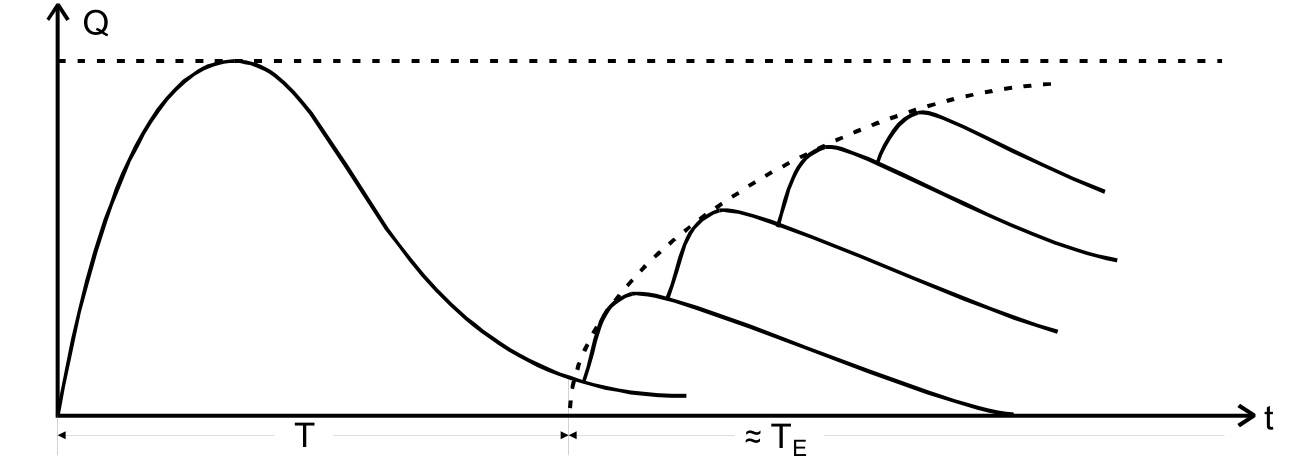
\includegraphics[width=0.8\textwidth]{content/data/totzeit.jpg}
    \caption{Die Totzeit $T$ und Erholungszeit $T_E$ eines Zählrohrs in einen $Q$-$T$-Diagramm dargestellt. \cite[4]{anleitung}}
    \label{fig:totzeit}
\end{figure}

\subsection{Charakteristik des Zählrohres}
Die Charakteristik hat die Gestalt wie in Abb. \ref{fig:charakteristik} zu sehen.
\begin{figure}
    \centering
    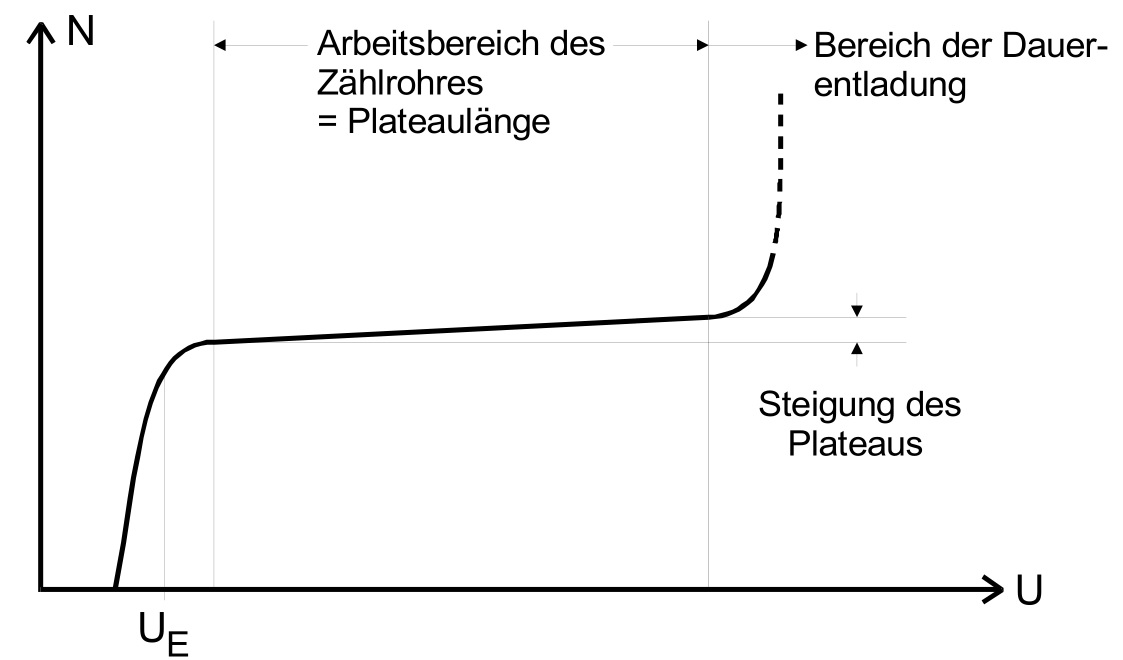
\includegraphics[width=0.8\textwidth]{content/data/charakteristik.jpg}
    \caption{Charakteristik eines Zählrohrs bei konstanter einfallender Strahlungsintensität. \cite[5]{anleitung}}
    \label{fig:charakteristik}
\end{figure}
Ab der Spannung $U_E$ beginnt der lineare Teil der Kurve (Plateau).
Die Steigung des Plateau wird durch Nachentladung verursacht, die trotz eines Alkoholdampfzusatzes entstehen.
Am Ende der Kurve nimmt die Anzahl der Nachentladungen stark zu.
Hier kann durch ein einzelnes ionisiertes Teilchen eine Dauerentladung beginnen.
Dabei treten hohe Stromdichten auf, welche das Zählrohr zerstören können (Bereich der Dauerentladung).
\\
Zur Untersuchung des Zählstroms wird die Zahl
\begin{equation}
    Z = \frac{I}{e_0 N}
    \label{eqn:Z}
\end{equation}
der freigesetzten Ladungen pro einfallende Teilchen benötigt.
$I$ entspricht hier dem gemessenen mittleren Zählrohrstrom, $N$ der Anzahl der einfallenden Teilchen und $e_0$ der Elementarladung.